\documentclass{beamer}	
\mode<presentation>
 
\usepackage{pdfpages}
\usepackage{fancyvrb}
\usepackage{chemarr}

\usepackage{amsmath}		%% mathematics typesetting
\usepackage{amssymb}
 
\usepackage{epigraph}   %% nice setting of quotations

\usepackage{tabularx} %% allows to use row colours in tables

\usepackage{ulem}

\usepackage{booktabs}

\usepackage{siunitx} %% tpyeset SI units

\usepackage{CJKutf8} %% typeset Chinese characters

\usepackage{pdfpages}%% include pdfs


\usepackage{animate} %% show animated gifs

\DeclareMathAlphabet{\mathcalligra}{T1}{calligra}{m}{n}


% Color and Theme. Can be changed. However, this one's quite nice.
\usetheme{Madrid}
\definecolor{theme}{rgb}{0.84,0,0.21}
\usecolortheme[named=theme]{structure}


%%  Title information
\title[M11.10.3 Schwangerschaft]{M11.10.3 Sexualentwicklung und Reproduktionsphysiologie II: Schwangerschaft}
\author[melanie.stefan@medicalschool-berlin.de]{}
\institute[]{Prof. Melanie Stefan - melanie.stefan@medcialschool-berlin.de}
\date{SoSe 2022}
 

% Table of contents to pop up at the beginning of each section
\AtBeginSection[]
{
  \begin{frame}<beamer>
    \frametitle{Outline}
    \tableofcontents[currentsection,currentsubsection]
  \end{frame}
}
 
\beamertemplatenavigationsymbolsempty

\begin{document}


{
  \usebackgroundtemplate{
\includegraphics[width=1.2\paperwidth]{MSB_Titelseite.pdf}} 
\begin{frame}

 \maketitle 

$\,$\\[6cm]


\end{frame} 
}



%% Hook: 

\begin{frame}

\begin{center}

\includegraphics[width=\textwidth]{supreme_court_abtreibung.png}
\end{center}

\end{frame} 



%% %% TLIA

 
\begin{frame}
\frametitle{In dieser Vorlesung geht es um\dots}


\begin{columns}[c]
\begin{column}{5cm}
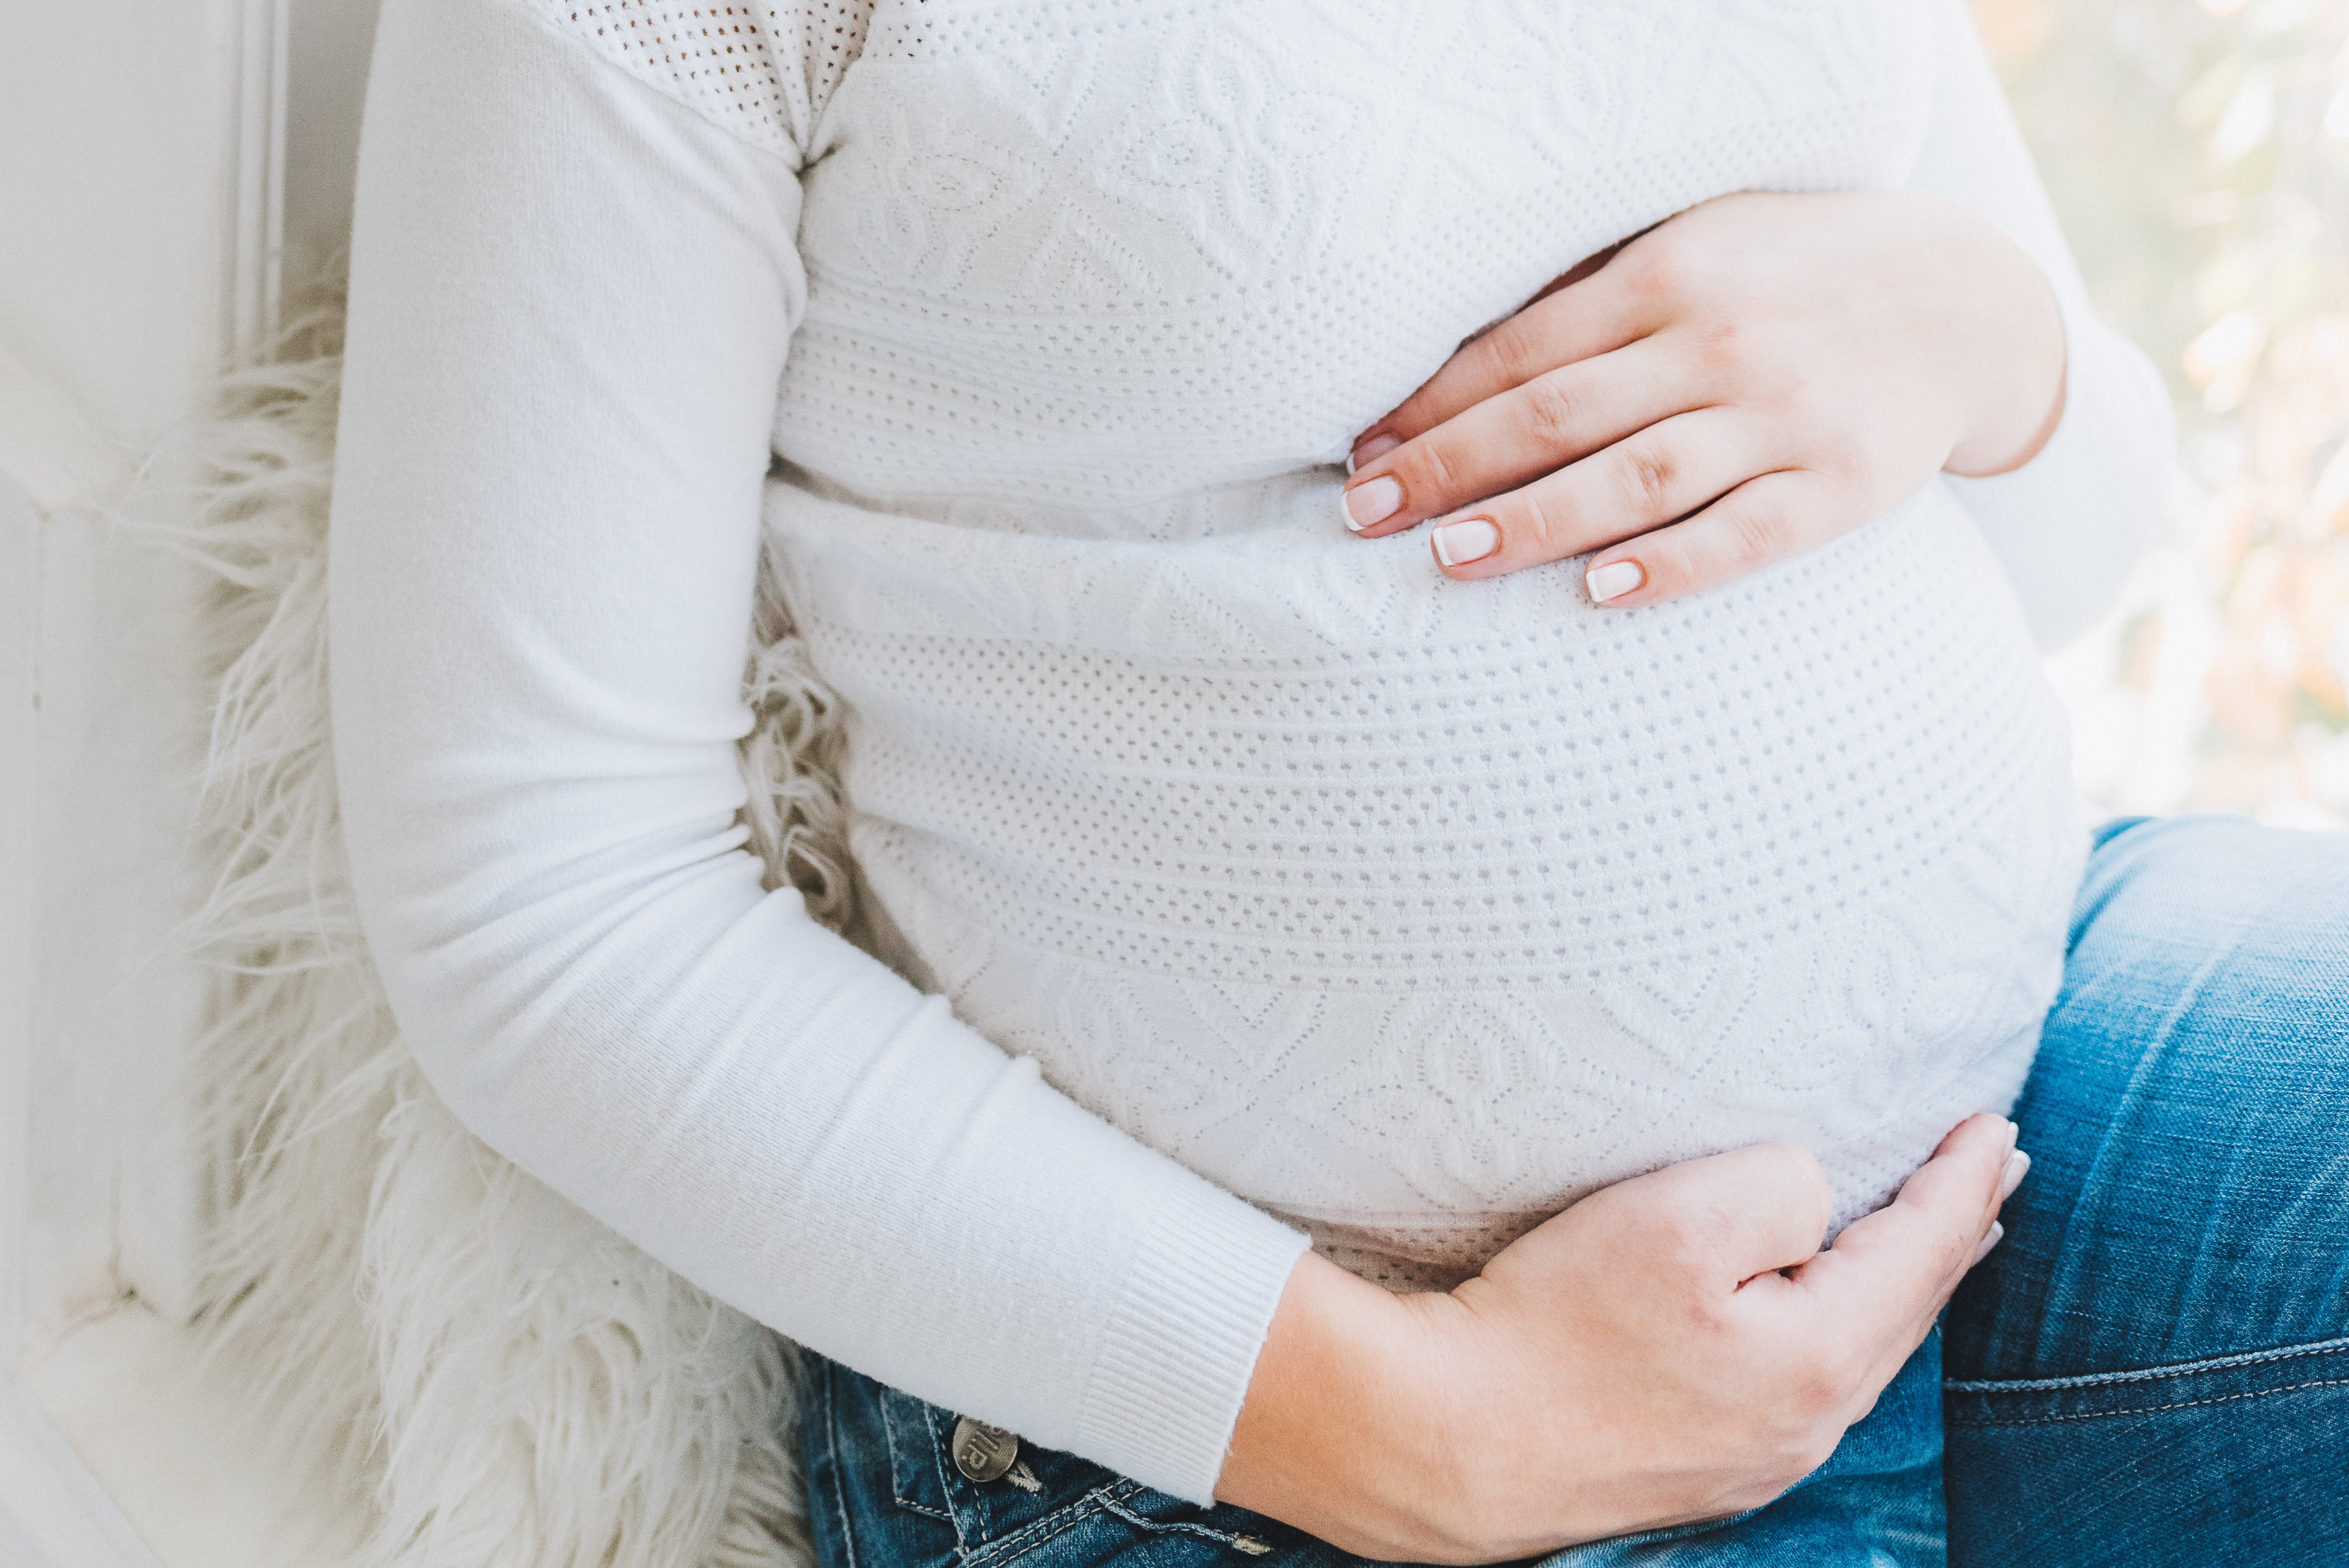
\includegraphics[width=\textwidth]{schwangerer_bauch.jpg}

\end{column}

\begin{column}{6cm}

\dots Schwangerschaft, \\ 
Entwicklung von Embryo und Fötus, \\
Geburt und Stillen

\end{column}
\end{columns}






\end{frame} 


%% %% Learning Objectives
 
\begin{frame}

 \frametitle{Nach dieser Vorlesung sollten Sie folgendes können}



\begin{block}{Grundlagen:}
\begin{itemize}
\item
Hormonelle Veränderungen im Verlauf der Schwangerschaft beschreiben und erklären
\item
die Entwicklung des Embryos und Foetus erklären 
\item
Körperfunktionen und Stoffaustausch des Fötus beschreiben
\item
die "Fetoplazentare Einheit" und Funktion der Plazenta erläutern
\item
den Geburtsvorgang beschreiben und erklären
\item
die hormonelle Steuerung der Laktation erklären

\end{itemize}

\end{block}



\begin{block}{Klinik:}
\begin{itemize}
\item
Erklären, wie ein Schwangerschaftstest funktioniert
\item
Häufige Beschwerden und Komplikationen in der Schwangerschaft erklären

\end{itemize}

\end{block}

\end{frame}


%% %% %% Main Body


\section{Schwangerschaft}

%% Befruchtung und nidation




\section{Entwicklung des Embryos und Fötus}


%% Embryonalentwicklung bis zur Einnistung
\begin{frame}
\frametitle{Während der ersten Zellteilungen wandert der Embryo in den Uterus}

\begin{center}
\includegraphics<1>[width=0.8\textwidth]{Human_Fertilization_Day0A.png}

\includegraphics<2>[width=0.8\textwidth]{Human_Fertilization_Day0B.png}

\includegraphics<3>[width=0.8\textwidth]{Human_Fertilization_Day0C.png}

\includegraphics<4>[width=0.8\textwidth]{Human_Fertilization_Day1.png}

\includegraphics<5>[width=0.8\textwidth]{Human_Fertilization_Day2.png}

\includegraphics<6>[width=0.8\textwidth]{Human_Fertilization_Day3A.png}

\includegraphics<7>[width=0.8\textwidth]{Human_Fertilization_Day3B.png}

\includegraphics<8>[width=0.8\textwidth]{Human_Fertilization_Day4.png}

\includegraphics<9>[width=0.8\textwidth]{Human_Fertilization_Day5.png}

\includegraphics<10>[width=0.8\textwidth]{Human_Fertilization_Day6.png}

\includegraphics<11>[width=0.8\textwidth]{Human_Fertilization.png}

\end{center}


\end{frame}


\begin{frame}
\frametitle{Komplikation: Ektopische Schwangerschaft im Eileiter}


\begin{columns}[c]
\begin{column}{5cm}

\begin{itemize}

\item
Embryo gelangt nicht in den Uterus, sondern nistet sich im Eileiter ein
\item
Wenn nicht erkannt,  kommt es  einem spontanen Abbruch oder einer (gefärhlichen) Eileiter-Ruptur
\item
Wenn erkannt, muss die Schwangerschaft beendet werden
\end{itemize}

\end{column}

\begin{column}{5cm}

\begin{center}
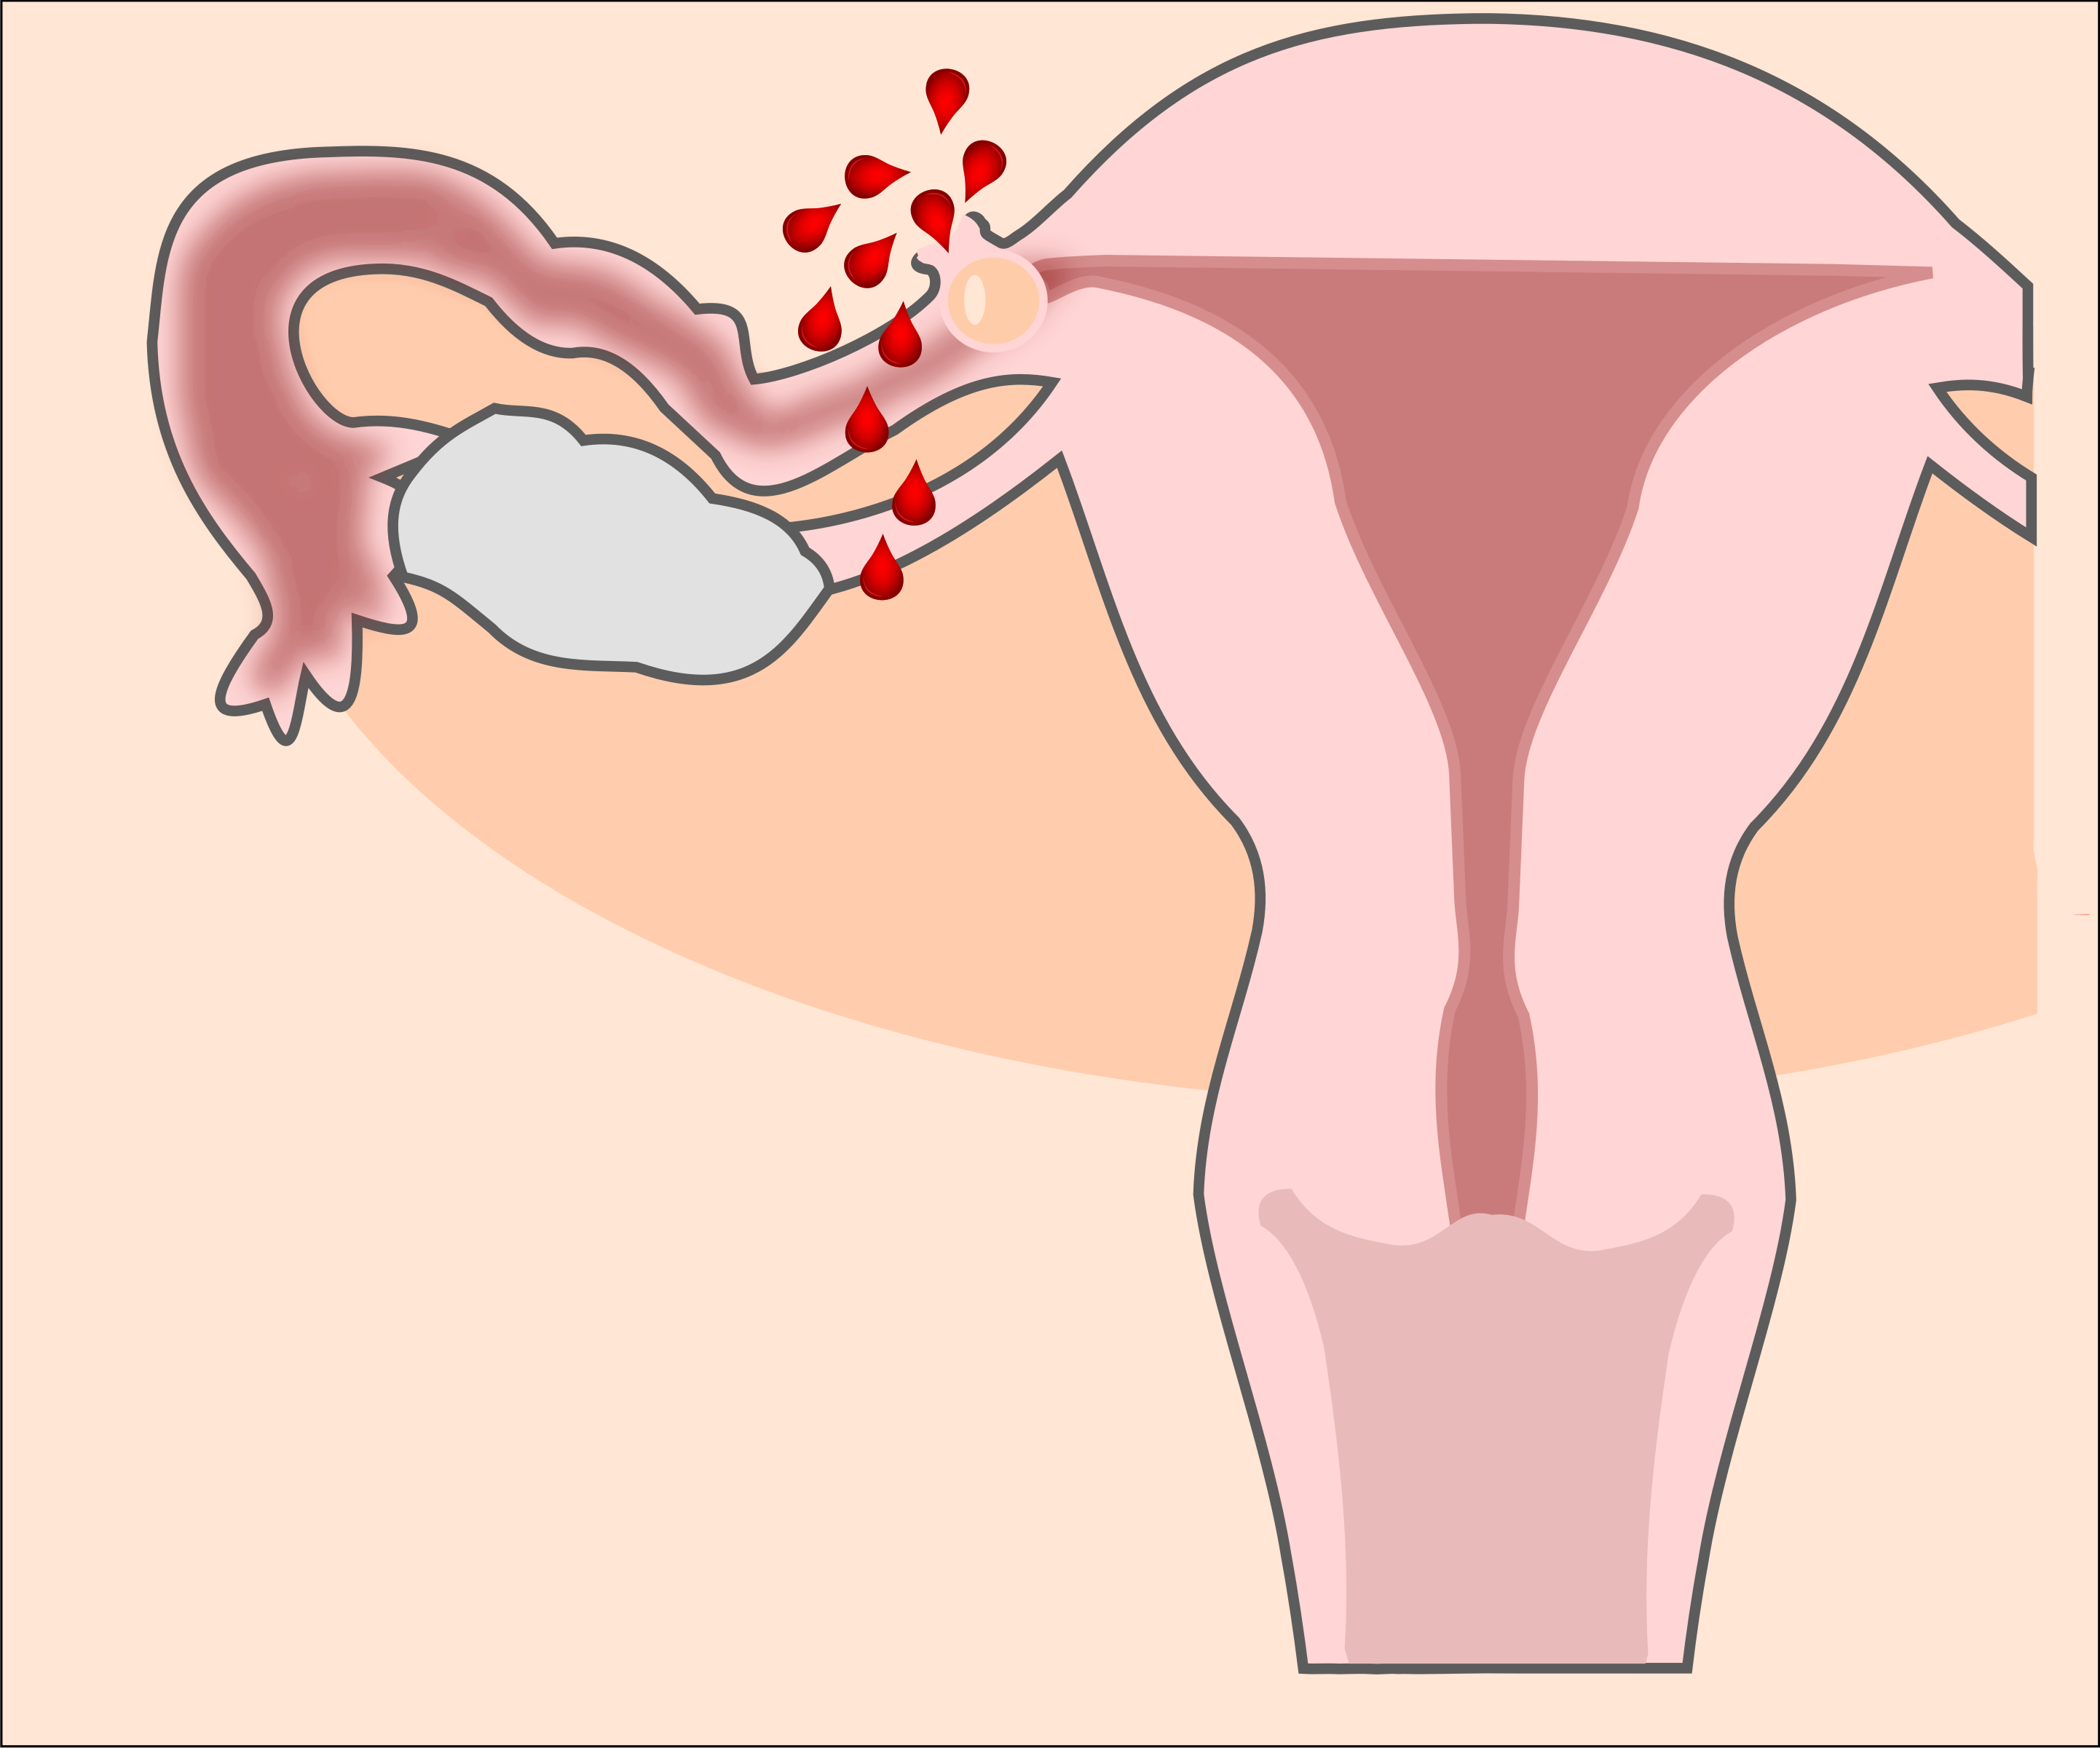
\includegraphics[width=\textwidth]{Eileiterruptur.png}
\end{center}


\end{column}
\end{columns}


\end{frame}



\section{Geburt}

\begin{frame}
\frametitle{Geburtsphasen }

\begin{block}{Einleitung}
\begin{itemize}
\item
Nach ca.  40 Schwangerschaftswochen
\item
Oxytozin- und Prostaglandine bewirken ein Einsetzen der Wehen
\end{itemize}
\end{block}


\begin{block}{Eröffnungsphase}
\begin{itemize}
\item
3-12 Stunden
\item
Wehen werden regelmäßiger
\item
Muttermund öffnet sich, Fruchtblase platzt
\end{itemize}
\end{block}


\begin{block}{Austreibungsphase}
\begin{itemize}
\item
1-2 Stunden
\item
Austreibungs- und Presswehen bringen das Kind durch den Geburtskanal
\end{itemize}
\end{block}


\end{frame}



\begin{frame}
\frametitle{Hormonelle Regelkreise ermöglichen die Geburt. }

\begin{center}
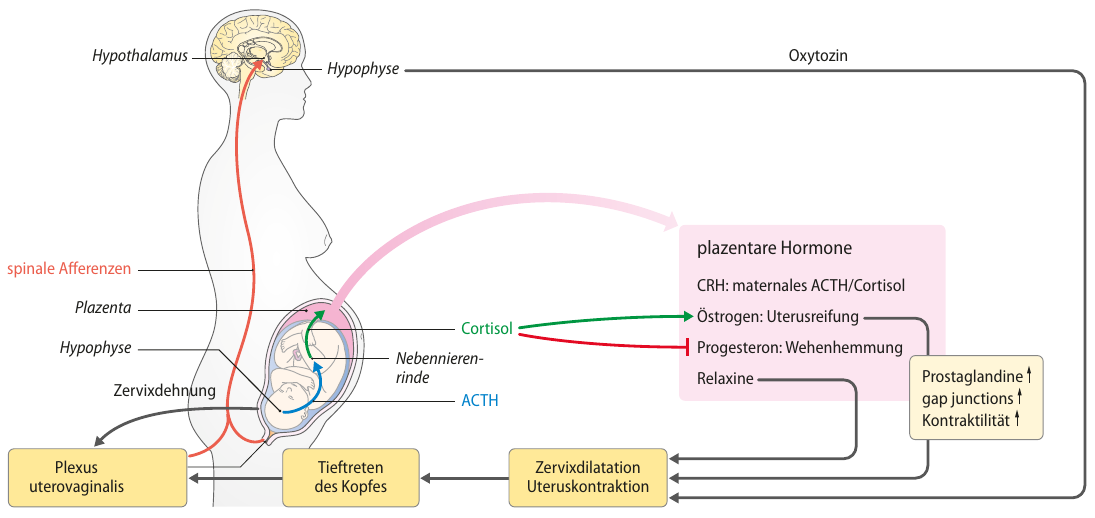
\includegraphics[width=\textwidth]{geburt_hormone}
\end{center}


\end{frame}

\section{Laktation}

%% Hormonelle Steuerung der Laktation

%% nicht Stillen ist auch ok - WHO Recommendations, Reality

%% Baby Formula Crisis



%% %% %% %% Review

\begin{frame}

\frametitle{Jetzt* sollten Sie folgendes können}

\end{frame}



%% %% %% %% Feedbackhinweisblock

\begin{frame}
\frametitle{Danke für Ihr Feedback!}

\begin{columns}[c]

\begin{column}{6cm}
\begin{center}
 
\includegraphics[width=\textwidth]{smilie_balloons.jpg}
\end{center}

\end{column}

\begin{column}{4cm}


\begin{center}

\includegraphics[width=\textwidth]{feedback_QR.png}
\end{center}
\end{column}


\end{columns}

\end{frame}



%% %% %% Bildnachweis
\begin{frame}
\frametitle{Bildnachweis}

\begin{tiny}
 
\begin{itemize}


\item
Bauch einer schwangeren Frau. Photo by \href{https://unsplash.com/es/@anastasiiachepinska?utm_source=unsplash&utm_medium=referral&utm_content=creditCopyText}{Anastasiia Chepinska} on \href{https://unsplash.com/s/photos/pregnancy?utm_source=unsplash&utm_medium=referral&utm_content=creditCopyText}{Unsplash}


\item
Befruchtung bis Einnistung im Menschen. Von Ttrue12, CC-BY-SA 3.0, 2012, Wikimedia Commons.

\item
Eileiter-Ruptur. Von Ectopic\_pregnancy.svg: Hic et nuncderivative work: Hic et nunc (talk) - Ectopic\_pregnancy.svg, CC BY-SA 3.0, \url{https://commons.wikimedia.org/w/index.php?curid=17236669}

\item
Hormonelle Regelkreise während der Geburt. Aus: Friederike Werny, Stefan Schlatt. Fetomaternale Interaktion, Geburt, Laktation. In: R. Brandes et al. (Hrsg.), Physiologie des Menschen, Springer-Lehrbuch \url{https://doi.org/10.1007/978-3-662-56468-4_81}


%% %% all lectures
\item
Luftballons mit frohen und traurigen Smilies. Photo by \href{https://unsplash.com/@artbyhybrid?utm_source=unsplash&utm_medium=referral&utm_content=creditCopyText}{Hybrid} on \href{https://unsplash.com/s/photos/feedback?utm_source=unsplash&utm_medium=referral&utm_content=creditCopyText}{Unsplash}

\item
Supreme Court will Recht auf Schwangerschaftsabbrüche abschaffen. Screenshot von Zeit Online, vom 3. Mai 2022.
\end{itemize}
\end{tiny}
\end{frame}





\end{document}


%%%% Columns - frequently used

%% \begin{columns}[c]
%% \begin{column}{5cm}

%% \end{column}

%% \begin{column}{5cm}

%% \end{column}
%% \end{columns}
